\documentclass[../main.tex]{subfiles}

\begin{document}

\subsection*{Exercice 1 :}
On considère le système suivant :
\[(S)= \left \{
   \begin{matrix}
   \dot{x} = \begin{pmatrix}-10 & 12\\-4 & 7\end{pmatrix} x_1 +  \begin{pmatrix} -1\\-1\end{pmatrix} u\\
   y_1 =\begin{pmatrix}4 & 5\end{pmatrix}x_1
   \end{matrix}
   \right.
\]
\begin{enumerate}
\item
\begin{enumerate}
\item Base modale \\
Déterminons les valeurs propres de la matrice d'évolution :\\
\begin{align*}
P(\lambda) &= det(A_1 - \lambda \mathbf{1}_2)\\
&= det \begin{pmatrix}-10-\lambda & 12 \\ -6 & 7 - \lambda \end{pmatrix}\\
&= (-10-\lambda)(7-\lambda)+72\\
&= -70 + 3\lambda + \lambda^2 +72\\
&= \lambda^2 +  3 \lambda +2\\
&= (\lambda + 1 )(\lambda + 2)
\end{align*}


Cherchons les vecteurs propres vérifiant $A_1X = \lambda X$:\\
Pour $\lambda = -1$ :
\begin{align*}
A_1X = \lambda X  &\rightarrow -6x_1 + 8x_2 =0
\end{align*}
On a donc :
\begin{align*}
E_{-1} &= Ker\{ -1. \mathbf{1}_3 - A\} \\
&= Vect\left \{ \begin{pmatrix}
4\\3
\end{pmatrix}\right \}
\end{align*}
\bigbreak
Pour $\lambda = -2$ :
\begin{align*}
A_1X = \lambda X  &\rightarrow -6x_1 + 9x_2 =0
\end{align*}
On a donc :
\begin{align*}
E_{-2} &= Ker\{ -2. \mathbf{1}_3 - A\} \\
&= Vect\left \{ \begin{pmatrix}
3\\2
\end{pmatrix}\right \}
\end{align*}
\bigbreak
La matrice de changement de base est donc : $P = \begin{pmatrix}4&3\\3&2\end{pmatrix}$\\
\item Le système est globalement asymptotiquement stable car les valeurs propres sont à $Re() < 0$.\\
On effectue alors le changement de base $x_1 = P \xi_1$

\begin{align*}
\left \{ \begin{matrix}
\dot{x}_1 = A_1+x_1 +B_1 u_1\\
y_1 = C_1 x_1
\end{matrix} \right. \rightarrow \left \{ \begin{matrix}
\dot{\xi}_1 = \Lambda\xi_1 + V^{-1}B_1u_1\\
y_1 = C_1V\xi_1
\end{matrix} \right.\\
\intertext{avec,} \Lambda = V^{-1}A_1V = \begin{pmatrix}
-1&0\\0&-2
\end{pmatrix}
\intertext{On a alors :}
\left \{\begin{matrix}
V^{-1}B_1 = \begin{pmatrix}-1\\1 \end{pmatrix} = B_m\\
C_1V = \begin{matrix}1&2\end{matrix} = C_m
\end{matrix} \right.
\end{align*}
\bigbreak

\item Rappel : pour $\dot{x} = Ax +Bu$ avec $x(0)=x_0 \in \mathbb{R}^n$ la solution est de la forme CI + régime forcé :
\[ x(t) = e^{At}x_0 + \int_0^te^{A(t-\tau)}Bu(\tau)d\tau\]
\bigbreak
Application :
\begin{align*}
\xi_1(t) &= e^{\Lambda t}\xi_0 + \int_0^te^{\Lambda (t-\tau)}B_mu_1(\tau)d\tau\\
e^{\Lambda t} &= e^{\begin{pmatrix}-t&0\\0&-2t\end{pmatrix}} = \begin{pmatrix}
e^{-t}&0\\0&e^{-2t}\end{pmatrix}\\
\xi_1(t) &= \begin{pmatrix}
\int_0^t -e^{-(t-\tau)}Bu(\tau)d\tau\\
\int_0^t e^{-2(t-\tau)}Bu(\tau)d\tau
\end{pmatrix}\\
y_1(t) &= C_m\xi_1(t)\\
&= \int_0^t -e^{-(t-\tau)}Bu(\tau)d\tau + \int_0^t 2e^{-2(t-\tau)}Bu(\tau)d\tau
&= \int_0^t (2e^{-2(t-\tau)}-e^{-(t-\tau)})Bu_1(\tau)d\tau
\end{align*}
Pour une réponse indicielle $u_1(t) = 1$ $\forall t \geq 0$\\

\item Commandabilité :
C(A,B) = $\begin{pmatrix}B & AB \end{pmatrix}$
\begin{align*}
A &= V\Lambda V^{-1}\\
B &= VB_m
\intertext{donc :}
C(A,B) &= \begin{pmatrix}VB_m &  V\Lambda V^{-1}VB_m \end{pmatrix}\\
&= \begin{pmatrix} VB_m &  V\Lambda B_m \end{pmatrix}\\
&= V \begin{pmatrix}B_m & \Lambda B_m \end{pmatrix}\\
&= V C(\Lambda,B_m)
\intertext{or,}
C(\Lambda,B_m) &= \begin{pmatrix}-1&1\\1&-2\end{pmatrix}\\
\text{donc, } det (C(\Lambda,B_m)) &= 1 \neq 0
\end{align*}
Ainsi, le système est commandable.\\

Remarque : Soit $x_1 \in \mathbb{R^2}$:
\begin{align*}
x_1(t) &= e^{A_1t}x_0 + \int_0^t e^{A_1(t-\tau)}B_1u_1(\tau)d\tau \in \mathbb{R^2}\\
W_c(0,t) &= \int_0^t e^{A_1(t-\tau)}B_1B_1^Te^{A_1^T(t-\tau)}d\tau \in \mathbb{R^{2*2}}\\
\intertext{$W_c(0,t_1)$ est inversible car commandable}
x_1(t_1) &= e^{A_1t_1}x_0 + \int_0^{t_1} e^{A_1(t_1-\tau)}B_1B_1^Te^{A_1^T(t_1-\tau)}W_c(0,t_1)^{-1}d\tau (x_1 - e^{A_1t_1}x_0) =x_1 \forall t_1 \geq 0\\
&= B_1e^{A(t_1-t)}W_c(0,t_1)^{-1}(x_1-e^{A_1t_1}x_0)
\end{align*}
\bigbreak
\end{enumerate}


\item On considère le système (S2) suivant :
\[(S2)= \left \{
   \begin{matrix}
   \dot{x}_2 = -10x_2 + 4u_2 & x_2(0) = x_0 \in \mathbb{R}^n\\
   y = -2x + u_2 &
   \end{matrix}
   \right.
\]

\begin{center}
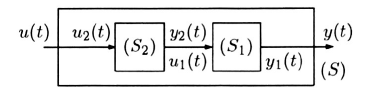
\includegraphics[scale=0.7]{TD7.png}
\end{center}
\bigbreak
\begin{enumerate}
\item La relation de connection est $u_1 = y_2$ et donne
\[\dot{\xi}_1 = \Lambda \xi_1 + B_m u_1 \text{	avec, } u_1 = y_2 = C_2x_2+ D_2u_2\]
D'où le système suivant :
\begin{align*}
\left \{ \begin{matrix}
\dot{\xi}_1 = \Lambda \xi_1 + B_mC_2x_2 + B_mD_2u_2\\
\dot{x}_2 = A_2x_2 + B_2u_2
\end{matrix} \right.
\end{align*}
Posons x(t) = $\begin{pmatrix}\xi_1\\x_2\end{pmatrix}$, on a alors :

\begin{align*}
\dot{x} &= \begin{pmatrix}
\Lambda & B_mC_2\\
0 & A_2
\end{pmatrix} x + \begin{pmatrix}
B_mD_2\\B_2
\end{pmatrix} u\\
\dot{x} &= \begin{pmatrix}
-1 & 0 & 2\\
0 & -2 & -2\\
0 & 0 &-10
\end{pmatrix} x + \begin{pmatrix}
-1 \\ 1 \\4 \end{pmatrix} u = Ax + Bu
\intertext{On a donc pour l'équation d'observation :}
y &= y_1 = C_m\xi_1 + D_1u_1\\
&= C_m \xi_1 + D_1y_2 \text{	où }D_1 = 0\\
&= C_m\xi_1\\
&= \begin{pmatrix}
1 & 2 & 0 \end{pmatrix}.\begin{pmatrix}
\xi_1 \\ x_2
\end{pmatrix}
\end{align*}

\item On regarde alors la commandabilité :
\begin{align*}
C(A,B) &= \begin{pmatrix} B & AB & A^2B \end{pmatrix}\\
&= \begin{pmatrix}
-1 & 9 & -89 \\
1 & -10 & 100\\
4 & -40 & 400
\end{pmatrix}\\
rang(C(A,B)) &= 2 \text{	car	} L_3 = 4L_2
\end{align*}

(S1) est stable, (S2) est stable mais l'association des deux ne l'est pas !\\

\item On considère le système (S) suivant :
\[(S)= \left \{
   \begin{matrix}
   \dot{x} = Ax + Bu & x(0) = x_0 \in \mathbb{R}^n\\
   y = Cx + Du &
   \end{matrix}
   \right.
\]
\noindent On introduit le vecteur :
\begin{align*}
\dot{x} &= \begin{pmatrix}
\dot{x}_1\\
\dot{x}_2\\
\vdots
\dot{x}_n\\
\end{pmatrix}
\intertext{et, sa transformée de Laplace}
L\{x\} &= \begin{pmatrix}
L\{x_1\}\\
L\{x_2\}\\
\vdots\\
L\{x_n\}\\
\end{pmatrix}\\
&= \begin{pmatrix}
X_1(p)\\
X_2(p)\\
\vdots\\
X_n(p)\\
\end{pmatrix} = X(p)
\intertext{on a alors avec le système (S)}
pX(p) -x_0 &= AX(p)+ BU(p)\\
(p\mathbf{1_n}-A)X(p) &= x_0 +BU(p)
\intertext{d'où la relation :}
X(p) &= (p\mathbf{1_n}-A)^{-1}BU(p) + (p\mathbf{1_n}-A)^{-1}x_0
\intertext{De même, on pose le vecteur :}
Y(p) &= L\{y(t)\}\\
&= CX(p) + DU(p)\\
&= [C(p\mathbf{1_n}-A)^{-1}B+D]u(p) + C(p\mathbf{1_n}-A)^{-1} x_0\\
&= G(p) U(p) + C(p\mathbf{1_n}-A)^{-1} x_0\\
\intertext{et on a :}
(p\mathbf{1_n}-A)^{-1} &= \frac{1}{det(p\mathbf{1_n}-A)} Adj(p\mathbf{1_n}-A)\\
G(p) &= \frac{C.Adj(p\mathbf{1_n}-A)B + DP_A(p)}{P_A(p)}
\end{align*}
Les pôles sont les modes.
On calcul donc :
\begin{align*}
p\mathbf{1_n}-A &= \begin{pmatrix}
p+1 & 0 & -2\\
0 & p+2 & 2\\
0 & 0 & p+10
\end{pmatrix}
\intertext{puis,}
(p\mathbf{1_n}-A)^{-1} &= \frac{1}{(p+1)(p+2)(p+10)}\begin{pmatrix}
(p+2)(p+10) & 0 & 0\\
0 & (p+1)(p+10) & 0\\
2(p+2) & -2(p+1) & (p+1)(p+2)
\end{pmatrix}^T
\intertext{ensuite,}
C(p\mathbf{1_n}-A)^{-1} &= \frac{1}{(p+1)(p+2)(p+10)} \begin{pmatrix}
(p+2)(p+10) & 2(p+1)(p+10) & 2(p+2)-4(p+1)
\end{pmatrix}
\intertext{enfin on obtient l'ordre 2 :}
C(p\mathbf{1_n}-A)^{-1}B &= G(p) = \frac{p}{(p+1)(p+10)}
\end{align*}
Remarque :
\begin{align*}
G(p) &= G_1(p) G_2(p)
\intertext{avec}
G_1(p) &= C_1(p\mathbf{1_2}-A_1)B_1 = \frac{p}{(p+1)(p+2)}\\
G_2(p) &= C_2(p\mathbf{1_1}-A_2)B_2 + D_2 = \frac{p+2}{p+10}
\end{align*}
Un pôle de $G_1$ a été neutralisé par un zéro de $G_2$, on a donc une perte de commandabilité.\\
Réalisation minimale : un vecteur d'état de taille la plus petite. Ici, ordre 2 (on avait un ordre 3 qui n'était pas minimal).
\end{enumerate}
\item On considère le système suivant :\\
\[\left \{ \begin{matrix}
\dot{x_1} &= &\begin{pmatrix}-10&12\\-6&7\end{pmatrix} x_1 &+ \begin{pmatrix}-1\\-1\end{pmatrix}\\
y_1 &= &\begin{pmatrix}4&-5\end{pmatrix}x_1
\end{matrix} \right.\]
\begin{enumerate}

\item On impose une trajectoire polynomiale : $y_d(t) = \sum_{k=0}^n \alpha_k \left(\frac{t}{T}\right)^k$\\
Avec les conditions initiales suivantes :\\ \smallbreak
\begin{center}
\begin{tabular}{|c|c|}
\hline
t=0 & t=T \\
\hline
\hline
$y_1(0)=0$ & $y_1(T)=1$ \\
\hline
$\dot{y_1}(0)=0$ & $\dot{y_1}(T)=0$ \\
\hline
$\ddot{y_1}(0)=0$ & $\ddot{y_1}(T)=0$ \\
\hline
\end{tabular}
\end{center}

On a aussi :
\begin{align*}
\dot{y_1}(t) &= \sum_{k=0}^n \frac{k}{T}\alpha_k \left(\frac{t}{T}\right)^{k-1}\\
\ddot{y_1}(t) &= \sum_{k=0}^n \frac{k(k-1)}{T^2}\alpha_k \left(\frac{t}{T}\right)^{k-2}\\
\end{align*}
\bigbreak

On a 6 contraintes donc 6 inconnues donc au maximum, $n=5$

\paragraph{à $t = 0$} :\\
\begin{align*}
y_1(0) &= \sum_{k=0}^5 \alpha_k \left(\frac{0}{T}\right)^k \Leftrightarrow \alpha_0 = 0\\
\dot{y_1}(0) &= \sum_{k=0}^5 \frac{k}{T}\alpha_k \left(\frac{0}{T}\right)^{k-1}  \Leftrightarrow \alpha_1 = 0\\
\ddot{y_1}(t) &= \sum_{k=0}^5 \frac{k(k-1)}{T^2}\alpha_k \left(\frac{0}{T}\right)^{k-2} \Leftrightarrow \alpha_2=0\\
\end{align*}

\paragraph{à $t = T$} :
\begin{align*}
y_1(T) = 1 &\Leftrightarrow \sum_{k=0}^5 \alpha_k = 1 \\
&\Leftrightarrow \alpha_3+\alpha_4 + \alpha_5 = 1\\
\dot{y_1}(T)=0 &\Leftrightarrow  \sum_{k=3}^5 \frac{k}{T}\alpha_k = 1 \\
&\Leftrightarrow \frac{1}{T}(3\alpha_3 + 4\alpha_4 + 5 \alpha_5) = 0\\
\ddot{y_1}(T) = 0 &\Leftrightarrow \sum_{k=3}^5 \frac{k(k-1)}{T^2}\alpha_k = 0 \\
&\Leftrightarrow \frac{1}{T^2}(6\alpha_3 + 12\alpha_4 + 20\alpha_5) = 0\\
\intertext{ce système est alors équivalent au calcul matriciel suivant :}
\begin{pmatrix}1&1&1\\3&4&5\\6&12&20\end{pmatrix}.\begin{pmatrix}\alpha_3\\ \alpha_4 \\ \alpha_5\end{pmatrix} &= \begin{pmatrix}1\\0\\0 \end{pmatrix}\\
\begin{pmatrix}\alpha_3\\ \alpha_4 \\ \alpha_5\end{pmatrix} &= \begin{pmatrix}1&1&1\\3&4&5\\6&12&20\end{pmatrix}^{-1}.\begin{pmatrix}1\\0\\0 \end{pmatrix}
\end{align*}

Le calcul abouti à :
\[\left \{\begin{matrix}
\alpha_3 = 10\\
\alpha_4 = -15\\
\alpha_5 = 6
\end{matrix} \right.\]

Remarque : On a une matrice 3x3, on peut donc se permettre de calculer l'inverse à partir des cofacteurs $\Delta_{ij} = (-1)^{i+j}|M_{ij}|$ avec $M_{ij}$ la matrice obtenu en supprimant la ligne i et la colonne j.\\

Remarque : $\ddot{y_1}(t)$ représente la secousse, aussi appelé Jerk.
Le quintique est la trajectoire à Jerk minimal.
\bigbreak
\bigbreak
\item Passage à la forme canonique de commandabilité.\\
Il s'agit de trouver la matrice de passage M du système d'état vers celui correspondant a $A_c$ une matrice compagnon horizontale de type 1 et $B_c$ un vecteur de 0 avec 1 sur la dernière composante. Puis, une fois que l'on à M, on calcule $C_c = M.C$\\

On a le polynôme caractéristique $P_{A_1}(\lambda) = \lambda^2 + 3\lambda + 2 = \lambda^2 + a_1\lambda + a_0$, dont on en déduit la matrice compagnon horizontale :
\[ A_c = \begin{pmatrix}
0&1\\-a_0&-a_1
\end{pmatrix} = \begin{pmatrix}
0&1\\-2&-3
\end{pmatrix}\]
Et on a aussi :
\[B_c = \begin{pmatrix}
0\\1\end{pmatrix}\]

Changement de coordonnées $M \in \mathbb{R}^{2x2}$ avec $M = \begin{pmatrix}m_1&m_2\end{pmatrix}$
\begin{align*}
M^{-1}AM = A_c &\Leftrightarrow AM = MA_c\\
&\Leftrightarrow\begin{pmatrix}
Am_1& Am_2
\end{pmatrix} = \begin{pmatrix}
m_1&m_2
\end{pmatrix}.\begin{pmatrix}
0&1\\-2&-3
\end{pmatrix}= \begin{pmatrix}
-2m_2& m_1 - 3m_2
\end{pmatrix}\\
&\Leftrightarrow \left\{ \begin{matrix}
Am_1 = -2m_2\\
Am_2 = m_1 - 3m_2
\end{matrix}\right.\\
&\Leftrightarrow \left \{ \begin{matrix}
 Am_1 = -2m_2\\
 (A+3\mathbf{1}_2)m_2 = m_1
\end{matrix}\right.
\intertext{or, $M^{-1}B = B_c\Leftrightarrow B=MB_c=m_2$, donc :}
M &= \begin{pmatrix}
B & (A+3\mathbf{1}_2)B
\end{pmatrix}
\intertext{d'où : }
M &= \begin{pmatrix}-5&-1\\-4&-1\end{pmatrix}
\end{align*}

Il est inutile de calculer $M^{-1}$ pour le calcul de la forme canonique. Car $C_c = C_1M = \begin{pmatrix}0&1\end{pmatrix}$ et, $D_c = D_1 = 0$
\item On impose $y_1(t) = 10\left(\frac{t}{T}\right)^3 - 15\left(\frac{t}{T}\right)^4 + 6\left(\frac{t}{T}\right)^5$.\\
On cherche une commande du type : $u_1(t) = \sum_{k=0}^m \beta_k \left(\frac{t}{T}\right)^k$.\\

\end{enumerate}
\paragraph{Forme de Browmovski }:

\begin{align*}
\begin{pmatrix}
\dot{z_1}\\\vdots\\\vdots\\\dot{z_n}\end{pmatrix} = \begin{pmatrix}
0&1&0&...&0\\
0&0&\ddots&&\\
0&...&...&1\\
-a_0&...&...&-a{n-1}
\end{pmatrix}.\begin{pmatrix}
z_1\\\vdots\\\vdots\\z_n
\end{pmatrix} + \begin{pmatrix}
0\\\vdots\\0\\1
\end{pmatrix}u
\end{align*}

Ayant la forme canonique de commandabilité, la forme de Browmovski conciste à poser :\\\[\boxed{v(t) = -a^Tz + u}\]
où $a = \begin{pmatrix}
a_0 &...&a_{n-1}
\end{pmatrix}^T$
d'où
\begin{align*}
\begin{pmatrix}
\dot{z_1}\\\vdots\\\vdots\\\dot{z_n}\end{pmatrix} = \begin{pmatrix}
0&1&0&...&0\\
0&0&\ddots&&\\
0&...&...&1\\
0&...&...&0
\end{pmatrix}.\begin{pmatrix}
z_1\\\vdots\\\vdots\\z_n
\end{pmatrix} + \begin{pmatrix}
0\\\vdots\\0\\1
\end{pmatrix}v
\end{align*}
Avec l'équation d'observation du système d'état $y = \begin{pmatrix}
c_0&...&c_{n-1}
\end{pmatrix}.\begin{pmatrix}
z_1\\\vdots\\z_{n-1}
\end{pmatrix}$

\paragraph{Application }:
Avec l'équation d'observation :
\begin{align*}
y_1 &= \begin{pmatrix}0&1\end{pmatrix} . \begin{pmatrix}z_1\\z_2\end{pmatrix} = z_2
\intertext{Puis, avec la forme de Brow***:}
&\left \{\begin{pmatrix}
\dot{z_1} = z_2\\
\dot{z_2} = v
\end{pmatrix}\right. \text{où $v= -\begin{pmatrix}
2&3
\end{pmatrix}\begin{pmatrix}
z_1\\z_2
\end{pmatrix} + u$}
\intertext{On a donc comme commande, en remplaçant avec les expressions provenant de l'équation d'obersation :}
u&= v + \begin{pmatrix}
2&3
\end{pmatrix}\begin{pmatrix}
z_1\\z_2
\end{pmatrix}
&=2z_1 + 3y_1 + \dot{y_1}\\
\intertext{On calcul donc chaque terme :}
z_1 &= \int_0^tz_2(\tau) d\tau\\
&= \int_0^ty_1(\tau) d\tau\\
&= \frac{10T}{4}\left(\frac{t}{T}\right)^4 -\frac{15T}{5}\left(\frac{t}{T}\right)^5 + \frac{6T}{6}\left(\frac{t}{T}\right)^6 + cst(=0)
\intertext{donc :}
u(t) &=2z_1 + 3y_1 + \dot{y_1}\\
&= 2T\left(\frac{t}{T}\right)^6 + (18-6T)\left(\frac{t}{T}\right)^5 + (\frac{30}{T}-45 + 5T) \left(\frac{t}{T}\right)^4 + (30-\frac{60}{T})\left(\frac{t}{T}\right)^3 + \frac{30}{T}\left(\frac{t}{T}\right)^2\\
&= \beta_6\left(\frac{t}{T}\right)^6 + \beta_5 \left(\frac{t}{T}\right)^5 + ...+\beta_2 \left(\frac{t}{T}\right)^2
\end{align*}

Donc m=6 et $\beta_1 = \beta_2 = 0$. Commande en boucle ouverte non robuste au conditions initiales. Il faut donc commander en boucle fermée.
\end{enumerate}


\end{document}
